% =====================================================================
%  Energy-Constrained UAV--UGV Replanning under Dynamic Road Conditions
%  Beamer source -- compile with pdflatex (run twice) or on Overleaf
% =====================================================================
\documentclass[aspectratio=169,10pt]{beamer}
\usetheme{default}
\usepackage[utf8]{inputenc}
\usepackage[T1]{fontenc}
\usepackage{lmodern}
\usepackage{amsmath,amssymb}
\usepackage{booktabs}
\usepackage{array}
\usepackage{pifont}
\usepackage{tikz}
\usetikzlibrary{arrows.meta,positioning,calc}
\hypersetup{colorlinks=true,urlcolor=blue}

% ----------------------- minimal visual identity -----------------------
\definecolor{Midnight}{HTML}{17324D}
\definecolor{Teal}{HTML}{159A96}
\definecolor{Amber}{HTML}{E8A93A}
\definecolor{Paper}{HTML}{F7F8FA}
\definecolor{Ink}{HTML}{202A35}
\definecolor{Muted}{HTML}{667085}

\setbeamertemplate{navigation symbols}{}
\setbeamertemplate{enumerate items}[default]
\setbeamertemplate{itemize item}{\color{Teal}\raise0.15ex\hbox{\scriptsize$\blacktriangleright$}}
\setbeamertemplate{itemize subitem}{\color{Teal}\raise0.1ex\hbox{\tiny$\blacktriangleright$}}

\setbeamercolor{background canvas}{bg=Paper}
\setbeamercolor{normal text}{fg=Ink,bg=Paper}
\setbeamercolor{structure}{fg=Teal}
\setbeamercolor{frametitle}{fg=Midnight,bg=Paper}
\setbeamercolor{title}{fg=Midnight}
\setbeamercolor{subtitle}{fg=Muted}
\setbeamercolor{author}{fg=Ink}
\setbeamercolor{institute}{fg=Muted}
\setbeamercolor{block title}{fg=white,bg=Midnight}
\setbeamercolor{block body}{fg=Ink,bg=white}
\setbeamercolor{block title alerted}{fg=white,bg=Amber!85!black}
\setbeamercolor{block body alerted}{fg=Ink,bg=Amber!10}
\setbeamercolor{footline}{fg=Muted,bg=Paper}

\setbeamerfont{title}{size=\Large,series=\bfseries}
\setbeamerfont{subtitle}{size=\large}
\setbeamerfont{frametitle}{size=\large,series=\bfseries}
\setbeamerfont{author}{size=\normalsize}
\setbeamerfont{institute}{size=\small}
\setbeamertemplate{blocks}[rounded][shadow=false]

% Subtle asymmetric background: a navy edge and two soft corner shapes.
\setbeamertemplate{background}{%
\begin{tikzpicture}[remember picture,overlay]
  \path[use as bounding box] (0,0) rectangle (0,0);
  \fill[Midnight] (current page.north west)
    rectangle ([xshift=1.4mm]current page.south west);
  \fill[Teal!8] ([xshift=-4mm,yshift=8mm]current page.north east)
    circle[radius=17mm];
  \fill[Amber!9] ([xshift=8mm,yshift=-5mm]current page.south east)
    circle[radius=14mm];
\end{tikzpicture}%
}

% Left-aligned title page with a short accent rule.
\setbeamertemplate{title page}{%
  \vspace*{0.9cm}
  \hspace*{0.5cm}%
  \begin{minipage}{0.88\textwidth}
    {\color{Teal}\rule{1.8cm}{2.4pt}}\par\vspace{5mm}
    {\usebeamerfont{title}\usebeamercolor[fg]{title}\inserttitle\par}
    \vspace{3mm}
    {\usebeamerfont{subtitle}\usebeamercolor[fg]{subtitle}\insertsubtitle\par}
    \vspace{8mm}
    {\color{Midnight!25}\rule{0.68\linewidth}{0.5pt}}\par\vspace{5mm}
    {\usebeamerfont{author}\usebeamercolor[fg]{author}\insertauthor\par}
    \vspace{2mm}
    {\usebeamerfont{institute}\usebeamercolor[fg]{institute}\insertinstitute\par}
  \end{minipage}
}

% Frame title with a short teal marker and a light horizontal rule.
\setbeamertemplate{frametitle}{%
  \nointerlineskip
  \vspace*{3.0mm}
  \hspace*{4mm}%
  \begin{beamercolorbox}[wd=0.89\paperwidth,sep=0pt]{frametitle}
    \strut\usebeamerfont{frametitle}\insertframetitle\strut
  \end{beamercolorbox}
  \hspace*{4mm}{\color{Teal}\rule{1.4cm}{1.5pt}%
  \color{Midnight!14}\rule{0.70\paperwidth}{0.5pt}}
}

% Compact footer: presentation label on the left, page number on the right.
\setbeamertemplate{footline}{%
  \leavevmode
  \begin{beamercolorbox}[wd=\paperwidth,ht=2.5ex,dp=1.1ex,
    leftskip=5mm,rightskip=5mm]{footline}
    \hfill\scriptsize\insertframenumber\,/\,\inserttotalframenumber
  \end{beamercolorbox}
}

\newcommand{\cmark}{\textcolor{green!50!black}{\ding{51}}}
\newcommand{\xmark}{\textcolor{red!70!black}{\ding{55}}}
\newcommand{\pmark}{\textcolor{orange!85!black}{$\sim$}}
\newcolumntype{P}[1]{>{\raggedright\arraybackslash}p{#1}}

% ------------------------------ title ----------------------------------
\title{Energy-Constrained UAV--UGV Replanning\\ under Dynamic Road Conditions}
\subtitle{Research Problem, Literature Review and Proposed Method}
\author{Mayank Anand \and Sudhanshu \and Sujal}
\institute{Department of Information Technology\\
Indian Institute of Information Technology, Allahabad}
\date{}

\begin{document}

% =====================================================================
\begin{frame}
  \titlepage
\end{frame}

% =====================================================================
\begin{frame}{Outline}
\begin{columns}[T]
\begin{column}{0.48\textwidth}
\begin{enumerate}
  \item Introduction
  \item Motivation
  \item Research Problem
  \item Literature Review
  \item Research Gap
\end{enumerate}
\end{column}
\begin{column}{0.48\textwidth}
\begin{enumerate}
  \setcounter{enumi}{5}
  \item Problem Statement
  \item Proposed Framework \& Research Methodology
  \item Conclusion \& Milestones
\end{enumerate}
\end{column}
\end{columns}
\end{frame}

% =====================================================================
\begin{frame}{1. Introduction: Heterogeneous UAV--UGV Teams}
\begin{columns}[T]
\begin{column}{0.54\textwidth}
\textbf{System overview}
\begin{itemize}
  \item UAVs visit tasks quickly, but their batteries have limited capacity.
  \item UGVs travel on roads and act as mobile charging stations.
  \item The plan must decide UAV task routes, UGV road routes and recharge meeting times.
  \item One UGV can recharge one UAV at a time.
  \item Roads may become blocked or slow because of debris, flooding or traffic.
\end{itemize}
\end{column}
\begin{column}{0.43\textwidth}
\textbf{Base environment (Mondal et al., 2025)}\\[1mm]
\scriptsize
\renewcommand{\arraystretch}{1.15}
\begin{tabular}{@{}ll@{}}
\toprule
Parameter & Value\\
\midrule
Workspace & 20 km $\times$ 20 km\\
UAV speed $v_a$ & 10 m/s\\
UGV speed $v_g$ & 4.5 m/s (roads only)\\
UAV fuel $F_a$ & 287.7 kJ\\
Power model & $P^a(v)=0.0461v^3-0.5834v^2$\\
 & $\quad-1.8761v+229.6$ W\\
Recharge time $T_R$ & constant per rendezvous\\
Failure penalty $\mathbb{P}$ & 800\\
Problem sizes & U15G5, U45G15 (+U60G20, U75G25)\\
Teams & 1U-1G, 2U-1G, 2U-2G, 4U-2G\\
\bottomrule
\end{tabular}
\end{column}
\end{columns}
\end{frame}

% =====================================================================
\begin{frame}{1. Introduction: The Base DRL Framework We Build On}
\begin{columns}[T]
\begin{column}{0.57\textwidth}
\scriptsize
\begin{itemize}\setlength{\itemsep}{0.6mm}
  \item \textbf{State:} current position, remaining fuel and visited tasks.
  \item \textbf{Action:} visit a task or go to a recharge point; infeasible actions are masked.
  \item \textbf{Objective:} each action incurs a time cost $r_t=t_{ij}+T_R$; mission cost is the maximum accumulated time across agents, plus a failure penalty.
  \item \textbf{Decoder:} two stages---(1) select the active agent, (2) select that agent's next task/recharge action.
  \item \textbf{Training:} REINFORCE learns the routing policy from simulator rollouts.
\end{itemize}
\vspace{-1mm}
\setlength{\fboxsep}{1.2mm}
\fcolorbox{Teal}{Teal!6}{%
  \parbox{0.92\linewidth}{%
  \textbf{Decoder}\quad
  $\rightarrow$ Agent selection: ``Who acts next?''\\[-0.2mm]
  \hspace*{12.5mm}$\rightarrow$ Action selection: ``What should that agent do?''\\[-0.2mm]
  \hspace*{12.5mm}$\rightarrow$ UAV: position + fuel + mission status\\[-0.2mm]
  \hspace*{12.5mm}$\rightarrow$ UGV: time + assigned UAV rendezvous information}}
\vspace{1mm}

{\tiny\textbf{Routing is learned;} UAV$\to$UGV support assignment is rule-based (greedy proximity).}
\end{column}
\begin{column}{0.40\textwidth}
\centering
\includegraphics[width=\linewidth,height=0.58\textheight,keepaspectratio]{prism-uploads/1.png}\\[1mm]
{\scriptsize Example UAV--UGV routes and recharge meeting points.}
\end{column}
\end{columns}
\end{frame}

% =====================================================================
\begin{frame}{2. Motivation}
\small
\begin{columns}[T]
\begin{column}{0.43\textwidth}
\textbf{Mission time and energy are different}
\begin{itemize}
  \item Mission time $T$ is the time taken by the last agent to finish.
  \item Energy $E$ is the total energy used by all UAVs.
  \item A faster plan can still use more energy.
\end{itemize}
\vspace{2mm}
\textbf{Roads can change}
\begin{itemize}
  \item The base paper assumes that all roads remain available.
  \item A blockage can delay the UGV and the planned recharge.
  \item The UAV may wait, use extra energy or miss the recharge.
\end{itemize}
\end{column}
\begin{column}{0.54\textwidth}
\centering
\includegraphics[width=\linewidth,height=0.62\textheight,keepaspectratio]{prism-uploads/Picture1.jpg}\\[2mm]
{\scriptsize A blocked road delays the UGV and increases UAV waiting energy.}
\end{column}
\end{columns}
\end{frame}

% =====================================================================
\begin{frame}{Illustrative Example: Mission Time vs. UAV Energy}
\footnotesize
\centering
\textbf{Scenario:} 2 UAVs + 1 UGV; same tasks and roads; both routes are battery-safe;
mission budget $B=230$ kJ.

\vspace{1mm}
\centering
\includegraphics[width=0.90\textwidth,height=0.47\textheight,keepaspectratio]
{prism-uploads/ChatGPT Image Sep 30, 2026, 01_07_52 PM.png}

\vspace{0.5mm}
\begin{columns}[c]
\begin{column}{0.22\textwidth}
\centering
\textbf{Policy A}\\[-1mm]
$300>230$ kJ\\
\textcolor{red!70!black}{Budget-infeasible}
\end{column}
\begin{column}{0.52\textwidth}
\centering
\setlength{\fboxsep}{2mm}
\fcolorbox{Teal}{Teal!7}{%
  \parbox{0.44\textwidth}{\centering
  \textbf{Key observation}\\[0.5mm]
  \normalsize $\text{3\% more time}\;\Rightarrow\;\text{26.7\% less UAV energy}$}}
\end{column}
\begin{column}{0.22\textwidth}
\centering
\textbf{Policy B}\\[-1mm]
$220\le230$ kJ\\
\textcolor{green!45!black}{Budget-feasible}
\end{column}
\end{columns}

\vspace{1mm}
{\tiny\color{Muted} Illustrative values for explaining the time--energy trade-off; not experimental results.}
\end{frame}

% =====================================================================
\begin{frame}{3. Research Problem}
\small
\begin{block}{Central question}
Can a learned UAV--UGV routing policy control total UAV energy and remain feasible when UGV roads
become blocked or slow during the mission?
\end{block}
\vspace{-1mm}
\scriptsize
\begin{columns}[T]
\begin{column}{0.49\textwidth}
\textbf{Research questions}
\begin{itemize}\setlength{\itemsep}{1mm}
  \item \textbf{RQ1:} What is the trade-off between mission time and UAV energy?
  \item \textbf{RQ2:} Can the proposed method keep energy within a given budget?
  \item \textbf{RQ3:} How do road blockages and delays affect time, energy and failures?
  \item \textbf{RQ4:} Can event-triggered replanning use fewer replans than periodic replanning?
\end{itemize}
\end{column}
\begin{column}{0.49\textwidth}
\textbf{Expected results to test}
\begin{itemize}\setlength{\itemsep}{1mm}
  \item \textbf{H1:} Energy can be reduced with only a small increase in mission time.
  \item \textbf{H2:} The constrained policy follows the energy budget better than a fixed penalty.
  \item \textbf{H3:} More road disruption causes more energy use and more failures.
  \item \textbf{H4:} Event-triggered replanning gives similar reliability with fewer replans.
\end{itemize}
\end{column}
\end{columns}
\end{frame}

% =====================================================================
\begin{frame}{4. Literature Review (1/2): Cooperative Routing}
\scriptsize
\setlength{\tabcolsep}{2pt}
\renewcommand{\arraystretch}{1.35}
\begin{tabular}{P{1.9cm}P{1.5cm}P{3.7cm}P{3.0cm}P{3.1cm}}
\toprule
\textbf{Paper} & \textbf{Year / publisher} & \textbf{Methodology} & \textbf{Dataset / setting} & \textbf{Performance measures}\\
\midrule
Maini et al. [3] & 2019, IEEE TAES & Two-stage planning using MILP and heuristics for one UAV and one road-based refuelling vehicle & Simulated coverage cases and field experiments & Coverage time, feasibility and computation time\\
\addlinespace
Fan et al. [6] & 2023, IEEE TVT & Deep reinforcement learning for a UAV using several charging stations & Simulated UAV routing cases & Route cost, solution quality and runtime\\
\addlinespace
\textbf{Mondal et al. [1]} & \textbf{2025, arXiv} & \textbf{Transformer DRL with sortie-wise planning for multiple UAVs and UGVs} & \textbf{U15G5, U45G15 and larger test cases} & \textbf{Mission time, gap, runtime and win rate}\\
\bottomrule
\end{tabular}

\vspace{3mm}
\footnotesize
\textbf{Main finding:} Mondal et al. [1] is the closest work because it supports multiple UAVs, multiple UGVs and mobile recharging.
\end{frame}

% =====================================================================
\begin{frame}{4. Literature Review (2/2): Energy and Uncertainty}
\scriptsize
\setlength{\tabcolsep}{2pt}
\renewcommand{\arraystretch}{1.35}
\begin{tabular}{P{1.9cm}P{1.5cm}P{3.7cm}P{3.0cm}P{3.1cm}}
\toprule
\textbf{Paper} & \textbf{Year / publisher} & \textbf{Methodology} & \textbf{Dataset / setting} & \textbf{Performance measures}\\
\midrule
Shi et al. [4] & 2022, IEEE CDC & Chance-constrained MDP for uncertain UAV fuel during a UAV--UGV meeting & Simulated mission with one UAV and one UGV & Expected travel time and battery-failure probability\\
\addlinespace
Lin et al. [5] & 2022, IEEE RA-L & Robust planning for UAV surveillance with mobile charging UGVs and unknown obstacles & Simulated surveillance environments & Maximum revisit time and energy feasibility\\
\addlinespace
Mondal et al. [2] & 2025, IEEE ICRA & Attention-based DRL with a risk limit for uncertain, wind-driven UAV fuel use & Simulated UAV--UGV routing cases & Mission time, fuel risk and success rate\\
\bottomrule
\end{tabular}

\vspace{3mm}
\footnotesize
\textbf{Main finding:} these papers study energy or uncertainty, but they do not combine a mission energy budget with roads that change during execution.
\end{frame}

% =====================================================================
\begin{frame}{5. Research Gap}
\footnotesize
\centering
\setlength{\tabcolsep}{4pt}
\renewcommand{\arraystretch}{1.2}
\begin{tabular}{P{3.4cm}ccccc}
\toprule
\textbf{Work} & \textbf{Learned} & \textbf{Multi UAV--UGV} & \textbf{Mission energy} & \textbf{UGV roads change} & \textbf{Online}\\
 & \textbf{policy} & & \textbf{budget} & \textbf{during execution} & \textbf{replanning}\\
\midrule
Mondal et al. [1] (base) & \cmark & \cmark & \xmark & \xmark & \pmark\ (tasks/team)\\
Ra-DRL [2] & \cmark & \pmark & \pmark\ (fuel risk) & \xmark & --\\
Shi et al. [4] & \xmark & \xmark & \pmark\ (fuel risk) & \xmark & \pmark\\
Lin et al. [5] & \xmark & \cmark & \pmark\ (feasibility) & \pmark\ (obstacles) & \pmark\\
\midrule
\textbf{This work} & \cmark & \cmark & \cmark & \cmark & \cmark\\
\bottomrule
\end{tabular}\\[1mm]
{\tiny \cmark\ addressed \quad \pmark\ partial \quad \xmark\ not addressed \quad -- not the focus}
\vspace{2mm}
\begin{block}{Gap statement}
\small
The reviewed work does not jointly study a learned multi-UAV--UGV policy, a total mission energy budget,
and replanning when UGV roads become blocked or slow.
\end{block}
\end{frame}

% =====================================================================
\begin{frame}{6. Problem Statement}
\small
\begin{block}{Goal}
Plan UAV and UGV routes that finish the mission quickly, keep total UAV energy within budget $B$,
and remain feasible when a road becomes blocked or slow.
\end{block}
\begin{columns}[T]
\begin{column}{0.52\textwidth}
\textbf{Simple formulation}
\[
\boxed{\text{Minimize mission time }T\quad\text{while}\quad E\le B}
\]
\begin{itemize}
  \item $T$: time when the last agent finishes.
  \item $E$: total energy used by all UAVs.
  \item $B$: allowed mission energy.
\end{itemize}
\end{column}
\begin{column}{0.45\textwidth}
\begin{alertblock}{Rules that must always hold}
\begin{itemize}
  \item Every task must be visited.
  \item Each UAV sortie must stay within its battery limit.
  \item A recharge meeting must use a reachable road node.
  \item One UGV recharges one UAV at a time.
\end{itemize}
\end{alertblock}
\end{column}
\end{columns}
\end{frame}

% =====================================================================
\begin{frame}{6. Road, Energy and Budget Models}
\small
\begin{columns}[T]
\begin{column}{0.49\textwidth}
\textbf{Road model}
\begin{itemize}
  \item \textbf{Normal edge:} use its original travel time.
  \item \textbf{Slow edge:} multiply travel time by $\kappa>1$.
  \item \textbf{Blocked edge:} remove it from the current UGV route.
\end{itemize}

\textbf{Event settings}
\begin{itemize}
  \item Type: blocked edge or slow edge.
  \item Level: low, medium or high.
  \item Time: early, middle or late in the mission.
  \item The policy learns about an event only when it occurs.
\end{itemize}
\end{column}
\begin{column}{0.49\textwidth}
\textbf{Energy model}
\[
E=\sum \big(P_{\text{fly}}t_{\text{fly}}+P_{\text{wait}}t_{\text{wait}}\big)
\]
\begin{itemize}
  \item Flying energy = flying power $\times$ flying time.
  \item Waiting energy is added only when the UAV waits in the air.
\end{itemize}

\textbf{Budget levels}
\[
B=\beta B_0,\qquad \beta\in\{0.70,0.80,0.90,1.00\}
\]
$B_0$ is the energy used by the base policy on the same static-road instance.
\end{column}
\end{columns}
\vspace{1mm}
\centering
\setlength{\fboxsep}{1.5mm}
\fcolorbox{Amber!85!black}{Amber!10}{%
  \parbox{0.88\textwidth}{\centering
  \makebox[0.48\linewidth][c]{\textbf{$F_a$: per-sortie battery feasibility}}\hfill
  \makebox[0.48\linewidth][c]{\textbf{$B$: mission-level cumulative energy budget}}\\[-0.2mm]
  \makebox[0.48\linewidth][c]{\scriptsize inherited from the base paper}\hfill
  \makebox[0.48\linewidth][c]{\scriptsize new project-level constraint}}}
\end{frame}

% =====================================================================
\begin{frame}{7. Proposed Framework: Architecture}
\centering
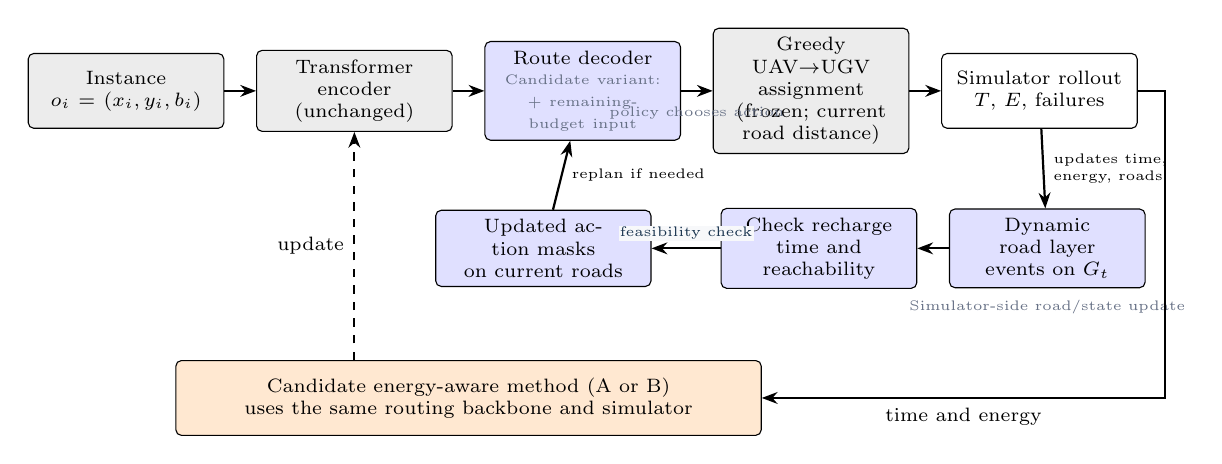
\begin{tikzpicture}[font=\scriptsize,
  box/.style={draw, rounded corners=2pt, align=center, text width=2.25cm, minimum height=0.95cm},
  fixed/.style={box, fill=gray!15},
  new/.style={box, fill=blue!12},
  train/.style={draw, rounded corners=2pt, align=center, fill=orange!18, text width=7.2cm, minimum height=0.95cm},
  a/.style={-{Stealth[length=2mm]}, thick}]
% top row
\node[fixed] (inst) at (0,2.3)    {Instance\\ $o_i=(x_i,y_i,b_i)$};
\node[fixed] (enc)  at (2.9,2.3)  {Transformer encoder\\ (unchanged)};
\node[new]   (dec)  at (5.8,2.3)  {Route decoder\\[-0.3mm]
  {\tiny\color{Muted}Candidate variant: + remaining-budget input}};
\node[fixed] (asg)  at (8.7,2.3)  {Greedy UAV$\to$UGV assignment\\ (frozen; current road distance)};
\node[box]   (env)  at (11.6,2.3) {Simulator rollout\\ $T$, $E$, failures};
% middle row
\node[new, text width=2.5cm] (mask) at (5.3,0.3)  {Updated action masks\\ on current roads};
\node[new] (mon)  at (8.8,0.3)  {Check recharge\\ time and reachability};
\node[new] (road) at (11.7,0.3) {Dynamic road layer\\ events on $G_t$};
\node[font=\tiny, text=Muted, align=center] at (11.7,-0.45)
  {Simulator-side road/state update};
% bottom row
\node[train] (tr) at (4.35,-1.6) {Candidate energy-aware method (A or B)\\
uses the same routing backbone and simulator};
% arrows
\draw[a] (inst) -- (enc);
\draw[a] (enc) -- (dec);
\draw[a] (dec) -- (asg);
\node[font=\tiny, text=Muted] at (7.25,2.02) {policy chooses action};
\draw[a] (asg) -- (env);
\draw[a] (env) -- node[right, align=left,font=\tiny]{updates time,\\energy, roads} (road);
\draw[a] (road) -- (mon);
\draw[a] (mon.west) -- node[midway,above=0.8mm,fill=Paper,
  inner sep=0.5pt,font=\tiny,text=Midnight]{feasibility check} (mask.east);
\draw[a] (mask) -- node[right,font=\tiny]{replan if needed} (dec);
\draw[a] (env.east) -- ++(0.35,0) |- node[pos=0.75, below]{time and energy} (tr.east);
\draw[a, dashed] (tr.north -| enc.south) -- node[left]{update} (enc.south);
\end{tikzpicture}\\[2mm]
{\scriptsize
\colorbox{gray!15}{\strut kept from base} \quad
\colorbox{blue!12}{\strut new / modified} \quad
\colorbox{orange!18}{\strut candidate method}}
\end{frame}

% =====================================================================
\begin{frame}{Two Candidate Energy-Aware Methods}
\footnotesize
\begin{columns}[T]
\begin{column}{0.48\textwidth}
\begin{block}{A. Lagrangian-Constrained Learning}
\scriptsize
\textbf{Keep the base decoder unchanged.}

\medskip
\textbf{Training score:}
\[
T+\lambda\max(0,E-B)
\]
\textbf{Update:}
\[
\lambda\leftarrow[\lambda+\eta(\bar E-B)]_+
\]
\textbf{Idea:} teach the policy to respect the mission-level energy budget through constrained optimization.
\end{block}
\end{column}
\begin{column}{0.48\textwidth}
\begin{block}{B. Budget-Conditioned Routing}
\scriptsize
\textbf{Add remaining mission budget to the decoder:}
\[
b_t=\frac{B-E_{\mathrm{used},t}}{B}
\]
Decoder receives current state + $b_t$.

\medskip
\textbf{Idea:} explicitly tell the policy how much mission energy remains when making each routing decision.
\end{block}
\end{column}
\end{columns}
\vspace{3mm}
\begin{block}{Fair comparison}
\centering
We compare A vs. B under the same environment, routing backbone, and frozen UAV$\to$UGV assignment.
\end{block}
\end{frame}

\begin{frame}{7. Proposed Framework: (B) Dynamic Roads \& Event-Triggered Replanning}
\small
\begin{columns}[T]
\begin{column}{0.58\textwidth}
\begin{block}{Event-triggered replanning}
\footnotesize
\begin{enumerate}
  \item Observe a blocked or slow road and update the road graph.
  \item Recompute the affected UGV path and arrival time.
  \item Check whether each planned recharge point is still reachable on time.
  \item If the current plan is still feasible, continue without replanning.
  \item Otherwise, keep the completed route and plan again for the remaining tasks.
\end{enumerate}
\end{block}
\end{column}
\begin{column}{0.39\textwidth}
\textbf{Replanning policies compared}
\begin{itemize}
  \item Open-loop (no replan)
  \item Periodic: at every recharge (as in the base case study)
  \item Event-triggered (ours)
\end{itemize}
\vspace{2mm}
\textbf{Training regimes}
\begin{itemize}
  \item Train only on static roads.
  \item Train with random road events.
\end{itemize}
\end{column}
\end{columns}
\vspace{1mm}
\begin{block}{Simulator--policy interface}
\scriptsize
The road graph is updated by the simulator; the same policy is queried again on the updated state when replanning is triggered.
\end{block}
\end{frame}

% =====================================================================
\begin{frame}{7. Research Methodology: Policies, Baselines \& Ablations}
\scriptsize
\centering
\renewcommand{\arraystretch}{1.18}
\begin{tabular}{P{3.2cm}P{4.2cm}P{6.0cm}}
\toprule
\textbf{Policy} & \textbf{Objective} & \textbf{What it tests}\\
\midrule
P0 Base & minimize $T$ & Original policy/reference\\
P1 Route filter & fastest route with $E\le B$ & Can post-hoc filtering work?\\
P2 Fixed penalty & minimize $T+\alpha E$ & Fixed reward shaping\\
P3 Lagrangian & minimize $T$ s.t.\ $E\le B$ & Candidate A: explicit constraint learning\\
P4 Budget-conditioned & budget-aware routing & Candidate B: remaining-budget conditioning\\
\bottomrule
\end{tabular}
\vspace{1.5mm}
\textbf{P3 and P4 are the two candidate methods investigated in this project.}
\vspace{1mm}
\begin{columns}[T]
\begin{column}{0.49\textwidth}
\textbf{Ablations}
\begin{itemize}\setlength{\itemsep}{0.4mm}
  \item Remove the remaining-budget input.
  \item Keep the energy penalty fixed.
  \item Compare no, periodic and event-triggered replanning.
\end{itemize}
\end{column}
\begin{column}{0.49\textwidth}
\vspace{3mm}
\begin{itemize}\setlength{\itemsep}{0.4mm}
  \item Train with and without random road events.
  \item Compare Euclidean and road distance for assignment.
\end{itemize}
\end{column}
\end{columns}
\end{frame}

% =====================================================================
\begin{frame}{7. Research Methodology: Experimental Design}
\small
\begin{columns}[T]
\begin{column}{0.45\textwidth}
\textbf{Experimental axes}\\[1mm]
\scriptsize
\renewcommand{\arraystretch}{1.2}
\begin{tabular}{@{}P{1.9cm}P{3.9cm}@{}}
\toprule
Axis & Values\\
\midrule
Energy budget & $0.70B_0,\ 0.80B_0,\ 0.90B_0,\ 1.00B_0$\\
Disruption & none, low, medium, high\\
Event timing & early, middle, late\\
Event type & edge blocked; travel time increased\\
Team size & 1U-1G, 2U-1G, 2U-2G, 4U-2G\\
Policies & P0--P4\\
\bottomrule
\end{tabular}\\[2mm]
\small Testing every combination is costly, so the experiments are divided into three stages.
\end{column}
\begin{column}{0.52\textwidth}
\textbf{Staged design}
\begin{itemize}
  \item \textbf{Stage A:} test energy budgets on static roads. This answers RQ1 and RQ2.
  \item \textbf{Stage B:} test blocked and slow roads. This answers RQ3 and RQ4.
  \item \textbf{Stage C:} test the best methods on larger problem sizes.
\end{itemize}
\textbf{Statistical protocol}
\begin{itemize}
  \item Use the same test cases and road events for every policy.
  \item Use 100 test instances and three training seeds.
  \item Report the mean, standard deviation and 95\% confidence interval.
\end{itemize}
\end{column}
\end{columns}
\end{frame}

% =====================================================================
\begin{frame}{7. Current Work: Gazebo Simulation \& Physics Validation}
\small
\begin{columns}[T]
\begin{column}{0.48\textwidth}
\textbf{Purpose of the testbed}
\begin{itemize}
  \item The routing model assumes travel time is distance divided by speed.
  \item Gazebo can show how terrain and wheel slip change the actual UGV arrival time.
  \item A late UGV may increase UAV waiting energy.
\end{itemize}
\textbf{Completed so far}
\begin{itemize}
  \item Desert terrain and a four-wheel UGV model are available.
  \item The UGV has a flat platform for UAV landing.
  \item The next step is to connect planned waypoints and road events to the simulator.
\end{itemize}
\end{column}
\begin{column}{0.49\textwidth}
\centering
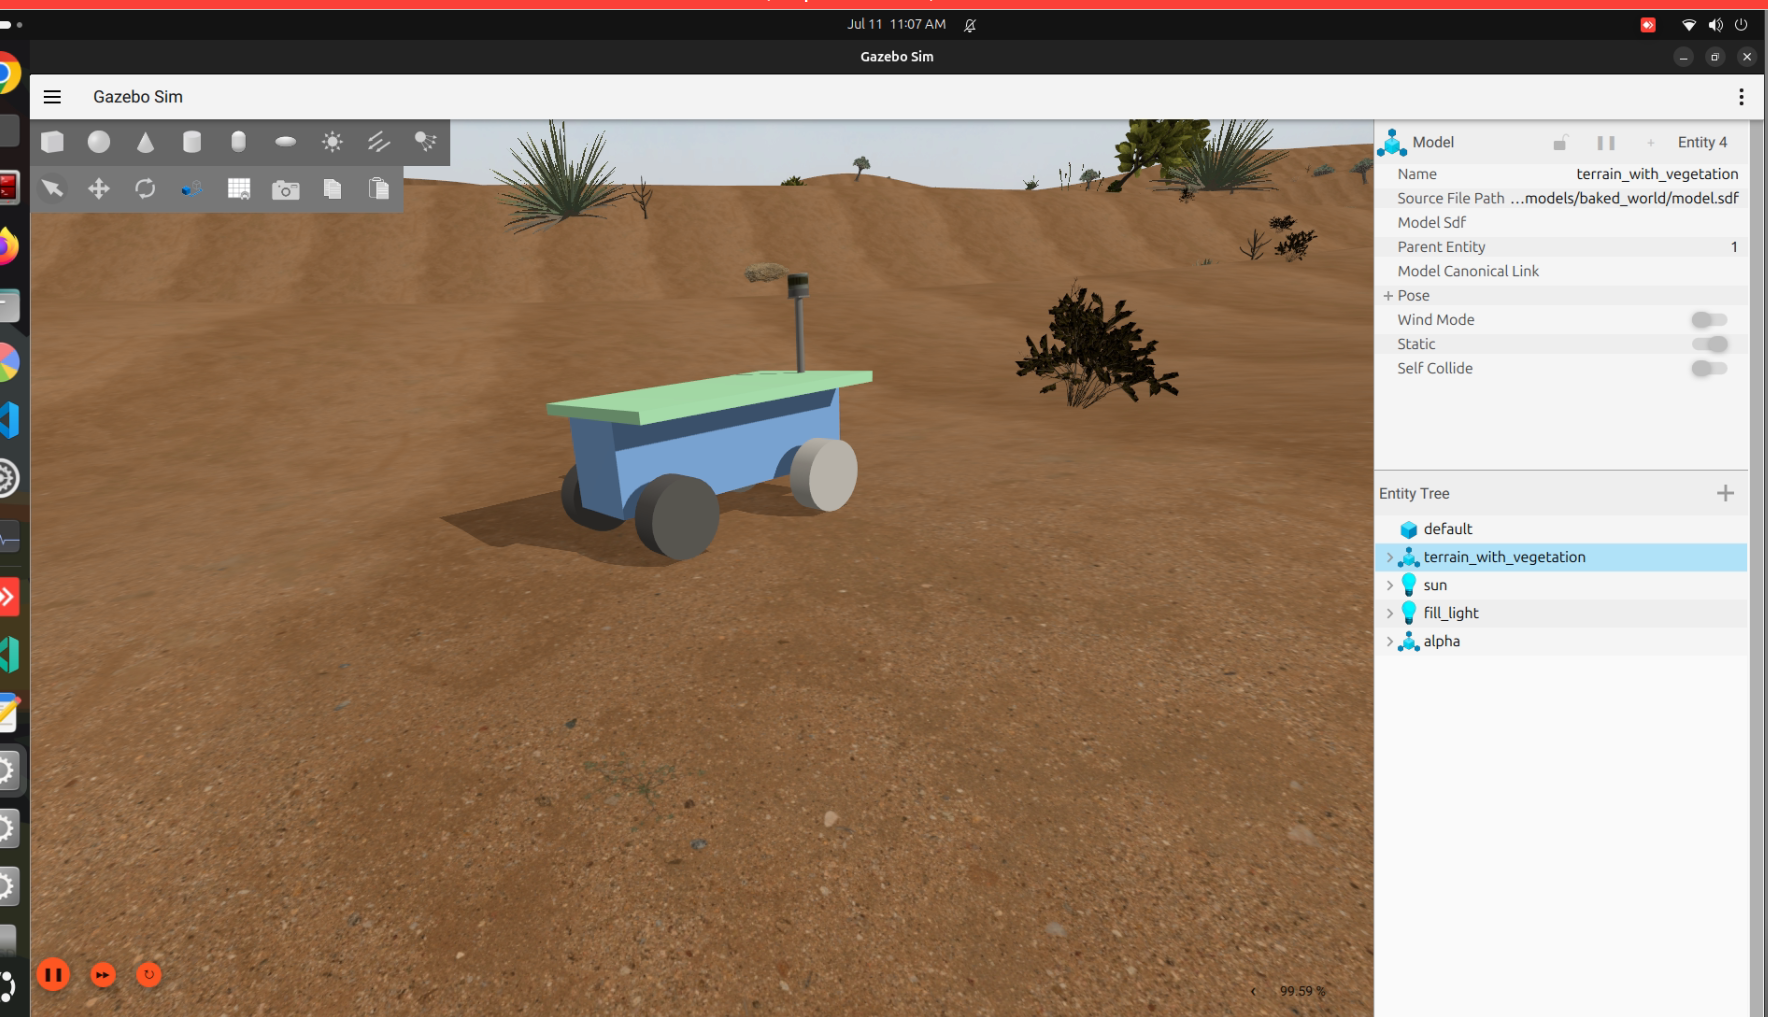
\includegraphics[width=\linewidth]{gazebo-ugv-desert.png}\\[1mm]
{\scriptsize UGV with landing pad traversing the desert terrain in Gazebo Sim.}
\vspace{2mm}
\begin{block}{Integration with this project}
\scriptsize
Send road waypoints to the UGV, add blocked or slow road segments, and record UGV arrival time and UAV waiting energy.
\end{block}
\end{column}
\end{columns}
\end{frame}

% =====================================================================
\begin{frame}{7. Research Methodology: Validation \& Risk Management}
\small
\begin{columns}[T]
\begin{column}{0.40\textwidth}
\textbf{Validation (Milestone 1)}
\begin{itemize}
  \item Reproduce base Table I trends (e.g.\ U15G5, 2U-1G greedy) within tolerance before any change.
  \item Hand-checkable cases: 1U-1G, 3 tasks; block the single edge to the next rendezvous $\Rightarrow$ verify reroute, ETA and mask.
  \item Unit test: $E=\sum P\cdot t$ per sortie; check how waiting is modelled (hover vs.\ landed).
\end{itemize}
\end{column}
\begin{column}{0.57\textwidth}
\scriptsize
\renewcommand{\arraystretch}{1.25}
\begin{tabular}{P{3.2cm}P{4.3cm}}
\toprule
\textbf{Risk} & \textbf{Mitigation}\\
\midrule
Energy and time may change together & measure both values and report the observed relation\\
Energy budget may be impossible & estimate the minimum possible energy before testing a budget\\
Energy penalty may be unstable & use a smaller update rate\\
Road graph may disconnect & first test blockages that keep an alternative path\\
Project scope may grow & keep the original assignment rule fixed\\
Base code or data may be incomplete & verify the base implementation before adding changes\\
\bottomrule
\end{tabular}
\end{column}
\end{columns}
\end{frame}

% =====================================================================
\begin{frame}{8. Conclusion \& Milestones}
\small
\begin{columns}[T]
\begin{column}{0.44\textwidth}
\textbf{Expected contribution}
\begin{itemize}
  \item Reproduce the base multi-UAV--UGV routing method.
  \item Add a total UAV energy budget without changing the base assignment rule.
  \item Add blocked and slow roads with event-triggered replanning.
  \item Measure mission time, energy use, budget violations and failures.
\end{itemize}
\end{column}
\begin{column}{0.53\textwidth}
\scriptsize
\renewcommand{\arraystretch}{1.25}
\begin{tabular}{P{0.6cm}P{3.1cm}P{3.0cm}}
\toprule
\textbf{M} & \textbf{Deliverable} & \textbf{Exit criterion}\\
\midrule
M1 & Reproduced base env + hand-checked cases & base trends reproduced; tests pass\\
M2 & Energy accounting; P0--P3 on static roads & RQ1/RQ2 answered; $\lambda$ converges\\
M3 & Dynamic road layer + event-triggered replanning & toy disruptions behave as expected\\
M4 & Ablations, seeds, scaling; final report & decision gate on dynamic-road effect (H3)\\
\bottomrule
\end{tabular}\\[2mm]
\small
\textbf{Final decision:} if road events have little effect, report that result and focus on the time--energy trade-off.
\end{column}
\end{columns}
\vspace{4mm}
\centering
\textbf{Thank you. Questions \& Discussion.}
\end{frame}

% =====================================================================
\begin{frame}{References}
\scriptsize
\begin{itemize}\setlength{\itemsep}{1.5mm}
  \item[{[1]}] M. S. Mondal, S. Ramasamy, L. Russo, J. D. Humann, J. M. Dotterweich, and P. Bhounsule,
  \href{https://arxiv.org/abs/2504.21111}{``How to coordinate UAVs and UGVs for efficient mission planning? Optimizing energy-constrained cooperative routing with a DRL framework,''} arXiv:2504.21111, 2025.

  \item[{[2]}] M. S. Mondal \emph{et al.}, \href{https://doi.org/10.1109/ICRA55743.2025.11128262}{``Risk-aware energy-constrained UAV--UGV cooperative routing using attention-guided reinforcement learning,''} in \emph{Proc. IEEE ICRA}, pp. 13000--13006, 2025.

  \item[{[3]}] P. Maini, K. Sundar, M. Singh, S. Rathinam, and P. B. Sujit, \href{https://doi.org/10.1109/TAES.2019.2917578}{``Cooperative aerial--ground vehicle route planning with fuel constraints for coverage applications,''} \emph{IEEE Trans. Aerosp. Electron. Syst.}, vol. 55, no. 6, pp. 3016--3028, 2019.

  \item[{[4]}] G. Shi \emph{et al.}, \href{https://doi.org/10.1109/CDC51059.2022.9993358}{``Risk-aware UAV--UGV rendezvous with chance-constrained Markov decision process,''} in \emph{Proc. IEEE CDC}, pp. 180--187, 2022.

  \item[{[5]}] X. Lin, Y. Yaz{\i}c{\i}o\u{g}lu, and D. Aksaray, \href{https://doi.org/10.1109/LRA.2022.3146938}{``Robust planning for persistent surveillance with energy-constrained UAVs and mobile charging stations,''} \emph{IEEE Robot. Autom. Lett.}, vol. 7, no. 2, pp. 4157--4164, 2022.

  \item[{[6]}] M. Fan \emph{et al.}, \href{https://doi.org/10.1109/TVT.2022.3232607}{``Deep reinforcement learning for UAV routing in the presence of multiple charging stations,''} \emph{IEEE Trans. Veh. Technol.}, vol. 72, no. 5, pp. 5732--5746, 2023.
\end{itemize}
\end{frame}

\end{document}